\documentclass{article}
\usepackage{listings}             % Include the listings-package
\usepackage[usenames,dvipsnames,svgnames,table]{xcolor}
\usepackage{graphicx}
\usepackage{hyperref}
\usepackage{amsmath}
\usepackage{amssymb}
\usepackage{amsthm}
\usepackage{csquotes}
\usepackage{changelog}
\usepackage{tabularx}
\usepackage{mathtools}
\usepackage{mdframed}
\usepackage{array}
\usepackage{float}
\usepackage{tikz}
\usepackage{soul}
\usepackage{makecell}
\usepackage{makeidx}
\usepackage{forest}

% Useful definitions for Math environments 
\newtheorem{theorem}{Theorem}[section]
\newtheorem{corollary}{Corollary}[theorem]
\newtheorem{lemma}[theorem]{Lemma}
\theoremstyle{definition}
\newtheorem{definition}{Definition}[section]
\newenvironment{remark}[1][Remark]{\begin{trivlist}
\item[\hskip \labelsep {\bfseries #1}]}{\end{trivlist}}

\newenvironment{dummy}{}{}

\definecolor{mygreen}{rgb}{0,0.6,0}
\definecolor{mygray}{rgb}{0.5,0.5,0.5}
\definecolor{mymauve}{rgb}{0.58,0,0.82}

\newcommand{\MrEHasherVersion}{0.1.0}
\newcommand{\FileColor}[1]{{\color{Purple} #1}}
\newcommand{\FolderColor}[1]{{\color{mygray} #1}}

\lstdefinelanguage{cmake} {morekeywords={one,two,three,four,five,six,seven,eight,
nine,ten,eleven,twelve,o,clock,rock,around,the,tonight}, sensitive=false,
morecomment=[l]{//},
morecomment=[s]{/*}{*/},
morestring=[b]", }

% Container for tabularx
\floatstyle{plain}
\newfloat{tabcontainer}{thp}{lop}
\floatname{tabcontainer}{Table}

% Container for tikz flow-charts
\floatstyle{plain}
\newfloat{fccontainer}{thp}{lop}
\floatname{fccontainer}{FlowChart}

% For visual representation of Flow-Charts
\usetikzlibrary{shapes.geometric, arrows}
\tikzstyle{startstop} = [rectangle, rounded corners, minimum width=3cm, minimum height=1cm,text centered, draw=black, fill=red!30]
\tikzstyle{process} = [rectangle, minimum width=3cm, minimum height=1cm, text centered, draw=black, fill=orange!30]
\tikzstyle{arrow} = [thick,->,>=stealth]
    
\title{MrEHasher}
\author{The\_Cowboy}
\pagestyle{headings}

\begin{document}

\maketitle
\tableofcontents

\lstset{language=Java}          % Set your language (you can change the language for each code-block optionally)

\bigskip


\section{Introduction}

\lstset{ %
  backgroundcolor=\color{white},   % choose the background color; you must add \usepackage{color} or    %\usepackage{xcolor}
  basicstyle=\footnotesize,        % the size of the fonts that are used for the code
  breakatwhitespace=false,         % sets if automatic breaks should only happen at whitespace
  breaklines=true,                 % sets automatic line breaking
  captionpos=b,                    % sets the caption-position to bottom
  commentstyle=\color{mygreen},    % comment style
  deletekeywords={...},            % if you want to delete keywords from the given language
  escapeinside={\%*}{*)},          % if you want to add LaTeX within your code
  extendedchars=true,              % lets you use non-ASCII characters; for 8-bits encodings only, %does not work with UTF-8
  frame=single,                    % adds a frame around the code
  keepspaces=true,                 % keeps spaces in text, useful for keeping indentation of code %(possibly needs columns=flexible)
  keywordstyle=\color{blue},       % keyword style
  language=Java,                 % the language of the code
  morekeywords={*,...},            % if you want to add more keywords to the set
  numbers=left,                    % where to put the line-numbers; possible values are (none, left, %right)
  numbersep=5pt,                   % how far the line-numbers are from the code
  numberstyle=\tiny\color{mygray}, % the style that is used for the line-numbers
  rulecolor=\color{black},         % if not set, the frame-color may be changed on line-breaks within %not-black text (e.g. comments (green here))
  showspaces=false,                % show spaces everywhere adding particular underscores; it %overrides 'showstringspaces'
  showstringspaces=false,          % underline spaces within strings only
  showtabs=false,                  % show tabs within strings adding particular underscores
  stepnumber=2,                    % the step between two line-numbers. If it's 1, each line will be %numbered
  stringstyle=\color{mymauve},     % string literal style
  tabsize=2,                       % sets default tabsize to 2 spaces
  title=\lstname                   % show the filename of files included with \lstinputlisting; also %try caption instead of title
} %optionally)

MrEHahser (version \MrEHasherVersion) is a native mod for generating the Turing Machine's electronics' data (for instance RAM serial number or CPU ID) and providing multiplatform access to unreal script.  Then the data can be utilized to compute hashes and associate with players' identiy in multiplayer gaming context. 

MrEHasher relies heavily upon a fork of the C library \href{https://github.com/ravimohan1991/BiosReader}{BiosReader} for querying electronics relevant information.

\section{Installation}
We will be leveraging latest NPLoader (version 19b) for installing MrEHasher in clients' Turing machines (computers).  Anthrax has already hinted that NPLoader may be replaced with better alternative in the future, till then, utilizing NPLoader is how we will proceed.
\begin{itemize}
\item Extract all the contents of \FolderColor{System} in your server's \FolderColor{System} directory.
\item Open \FileColor{UnrealTournament.ini} (or, depending upon server setting, \FileColor{Server.ini}).
\item Add the following server actor (be careful while copying the `\_' underscore from pdf, if opted)\\
\fbox{%
    \parbox{\textwidth}{%
       [Engine.GameEngine]\\
       \ldots \\
       ServerActors=NPLoader\_v19b.NPLActor\\
       \ldots
    }
}
\\
Discard this step if you have already installed latest ACE with NPLoader 19b.
\item Add the section (again, look out for `\_' underscores) \\

\fbox{%
    \parbox{\textwidth}{%
       [NPLoader\_v19b.NPLActor]\\
       bAutoInstallNewMods=True\\
       bAutoFixInstalls=True\\
       bUseNativeHelper=False\\
       PackageHelperClass=PackageHelper\_v15.PHActor\\
       ModInfoClasses[0]=MrEHasher.NPInfo\\
    }
}
\\
\item If you already have NPLoader's ModInfoClasses[0] filled already, fill the next empty entry, which in this instane would be like\\

\fbox{%
    \parbox{\textwidth}{%
       [NPLoader\_v19b.NPLActor]\\
       bAutoInstallNewMods=True\\
       bAutoFixInstalls=True\\
       bUseNativeHelper=False\\
       PackageHelperClass=PackageHelper\_v15.PHActor\\
       ModInfoClasses[0]=SomePackage.SomeStuff\\
       {\color{Green}ModInfoClasses[1]=MrEHasher.NPInfo}\\
    }
}
\\

\item And you are done. NPLoader shall take over and fill up the relevant ServerActors and ServerPackages automatically with reboot and all that!!
\item Finally start your server with the command line like so (without quotes)\\
``ucc server CTF-Face.unr?game=Botpack.CTFGame?mutator=MrEHasher.MrEMutator''

\end{itemize}

\section{Compiling}
In this section, I shall explain how to compile MrEHasher from source in Windows.  Ensure that you have latest version of Microsoft Visual Studio and WotGreal (optional). The mod has 
been split into two components

\begin{itemize}
\item Server Components
\begin{itemize}
\item \FileColor{MrEHasher.u}
\item \FileColor{MrEHasher\_Client.dll}
\item \FileColor{MrEHasher\_Client.u}
\item \FileColor{MrEHasherdll\_Client.u}
\end{itemize}
\item Client Components
\begin{itemize}
\item \FileColor{MrEHasher\_Client.dll}
\item \FileColor{MrEHasher\_Client.u}
\item \FileColor{MrEHasherdll\_Client.u}
\end{itemize}
\end{itemize}

\subsection{Few Words For Mod Authors}
If the instructions of are not followed this way, an imminent crash, figure \ref{fig:nativebindcrash}, can be observed in some situations.  This is because ``ULinker'' can't find the relevant function declarations if the class has been already spwned on the server and client hasn't installed the mod, or, to be specific, \FileColor{MrEHasher\_Client.dll} yet.

\begin{figure}
\centering
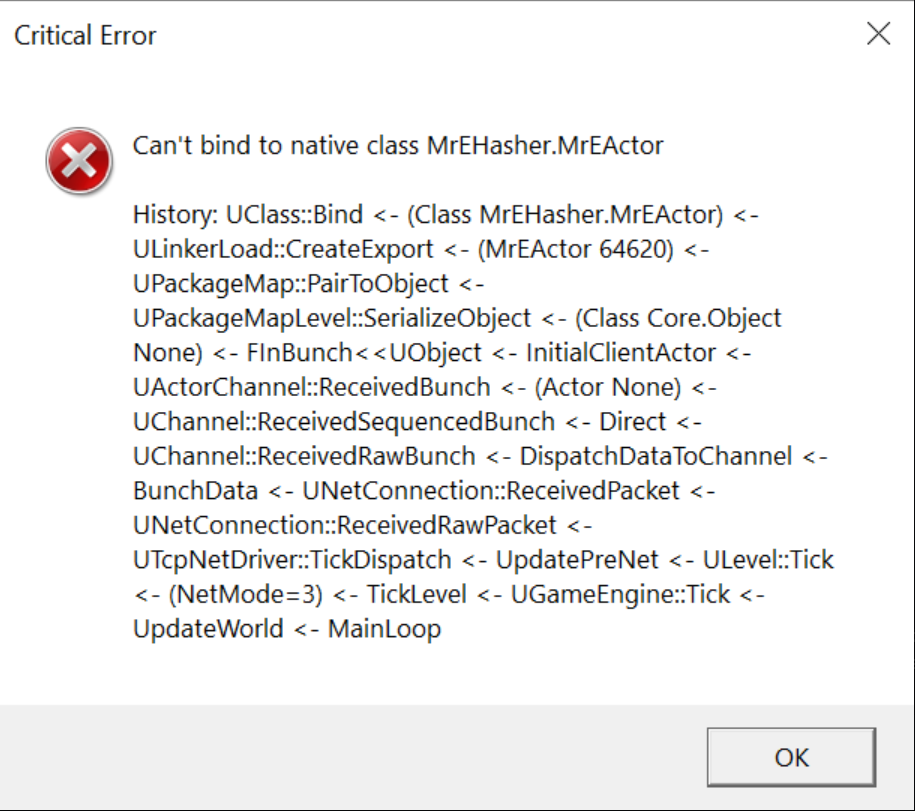
\includegraphics[width=0.4\textwidth]{img_nativebindcrash}
\caption{Crash notice}
\label{fig:nativebindcrash}
\end{figure}



\section{Understanding Native Code}
\end{document}